\documentclass{article}

\usepackage{graphicx}
\usepackage{tikz}
\usepackage{tikzsymbols}
\usetikzlibrary{calc,patterns,shapes.geometric}
\pagestyle{empty}
\usepackage[margin=0pt]{geometry}
\geometry{papersize={14in,12in}}

\def\centerarc[#1](#2)(#3:#4:#5){\draw[#1] ($(#2)+({#5*cos(#3)},{#5*sin(#3)})$) arc (#3:#4:#5);}

\begin{document}
	\begin{figure}
		\centering
		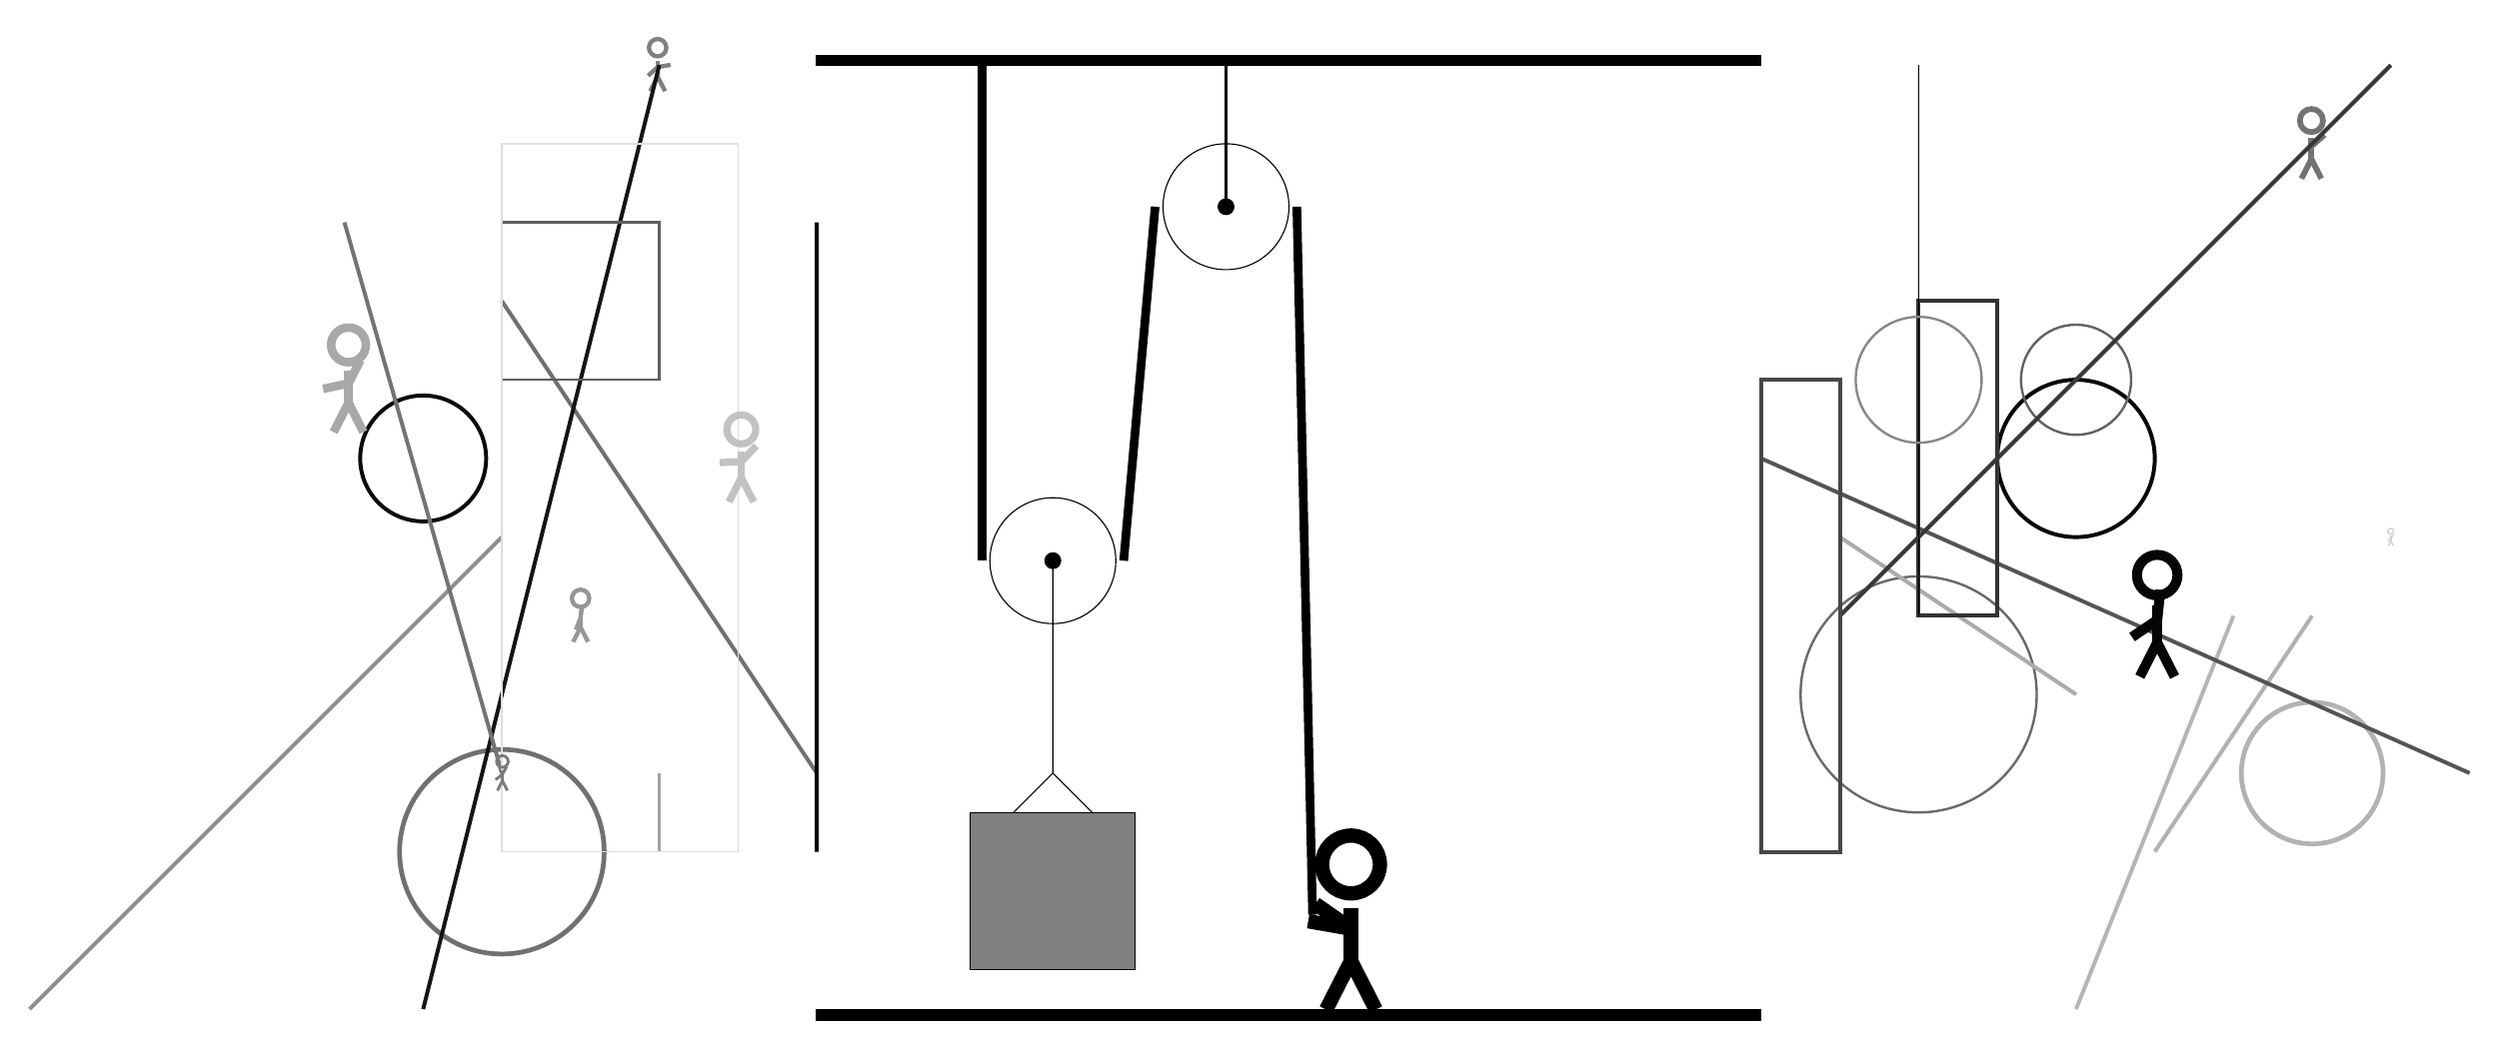
\begin{tikzpicture}
			%%%%% START %%%%%
			
			\draw[fill=black] (-2, 9) rectangle (10, 9.125);
			
			\draw [line width=0.5mm, color=black!96](-7, 4) circle (0.8);
			
			\draw [line width=0.6mm, color=black!56](-6, -1) circle (1.3);
			\draw [line width=0.3mm, color=black!59](12, 1) circle (1.5);
			\draw[line width=0.5mm, color=black!56](-2, 0) -- (-6, 6);
			
			\draw [line width=0.5mm, color=black!98](14, 4) circle (1.0);
			\node[line width=0.5mm, color=black!50] at (-4, 9) {\Strichmaxerl[3][43][9]};
			\draw[line width=0.5mm, color=black!92](-7, -3) -- (-4, 9);
			
			\draw [line width=0.6mm, color=black!30](17, 0) circle (0.9);
			\draw [line width=0.3mm, color=black!62](14, 5) circle (0.7);
			\draw[line width=0.5mm, color=black!29](14, -3) -- (16, 2);
			
			\node[line width=0.4mm, color=black!41] at (-5, 2) {\Strichmaxerl[3][69][83]};
			
			\draw[line width=0.3mm, color=black!36] (-4, 0) rectangle (-4, -1);
			\draw[line width=0.5mm, color=black!44](-6, 3) -- (-12, -3);
			
			\draw[line width=0.5mm, color=black!30](15, -1) -- (17, 2);
			\draw [line width=0.2mm, color=black!90](10, 7) circle (0.0);
			\draw[line width=0.4mm, color=black!100] (-2, 7) rectangle (-2, -1);
			
			\draw[line width=0.5mm, color=black!67](10, 4) -- (19, 0);
			
			\node[line width=0.6mm, color=black!34] at (-8, 5) {\Strichmaxerl[6][12][63]};
			\draw[line width=0.5mm, color=black!55](-6, 0) -- (-8, 7);
			\draw[line width=0.5mm, color=black!33](11, 3) -- (14, 1);
			\draw[line width=0.3mm, color=black!63] (-4, 5) rectangle (-6, 7);
			
			\node[line width=0.6mm, color=black!98] at (15, 2) {\Strichmaxerl[7][34][84]};
			\draw[line width=0.2mm, color=black!13] (-3, -1) rectangle (-6, 8);
			\draw[line width=0.5mm, color=black!80] (12, 2) rectangle (13, 6);
			\node[line width=0.3mm, color=black!24] at (-3, 4) {\Strichmaxerl[5][3][46]};
			\node[line width=0.2mm, color=black!55] at (17, 8) {\Strichmaxerl[4][90][41]};
			
			\draw[line width=0.5mm, color=black!78](11, 2) -- (18, 9);
			\node[line width=0.4mm, color=black!18] at (18, 3) {\Strichmaxerl[1][50][47]};
			\node[line width=0.5mm, color=black!52] at (-6, 0) {\Strichmaxerl[2][38][61]};
			\draw[line width=0.2mm, color=black!100] (12, 9) rectangle (12, 2);
			\draw[line width=0.5mm, color=black!72] (10, 5) rectangle (11, -1);
			
			\draw [line width=0.3mm, color=black!47](12, 5) circle (0.8);
			
			\draw (3.2, 7.2) circle (0.8);
			\draw[fill=black] (3.2, 7.2) circle (0.1);
			\draw[thick] (3.2, 7.2) -- (3.2, 9);
			
			\draw (1, 2.7) circle (0.8);
			\draw[fill=black] (1, 2.7) circle (0.1);
			
			\draw (1, 2.7) -- (1, 0) -- (0.5, -0.5);
			\draw (1, 0) -- (1.5, -0.5);
			\draw[fill=black!50] (-0.05, -0.5) rectangle (2.05, -2.5);
			
			\draw[line width=1.1mm] (0.1, 9) -- (0.1, 2.7);
			\centerarc[line width=1.1mm](1, 2.7)(180:360:0.9);
			\draw[line width=1.1mm](1.9, 2.7) -- (2.3, 7.2);
			\centerarc[line width=1.1mm](3.2, 7.2)(0:180:0.9);
			\draw[line width=1.1mm](4.1, 7.2) -- (4.3, -1.8);
			
			\node at (4.7, -1.9) {\Strichmaxerl[10][-35][170]};
			
			\draw[fill=black] (-2, -3) rectangle (10, -3.15);
			
			%%%%% END %%%%%
		\end{tikzpicture}
	\end{figure}	
\end{document}